% !TeX program = pdflatex
\documentclass[11pt,a4paper]{article}

% \usepackage{lmodern}  % descomente se disponivel (Overleaf tem)
\usepackage[T1]{fontenc}
\usepackage[utf8]{inputenc}
% Se o seu TeX tiver o babel em portugues (Overleaf tem), descomente:
% \usepackage[brazil]{babel}
\usepackage[margin=2.7cm]{geometry}
\usepackage{amsmath,amssymb,amsthm}
\usepackage{mathtools}
\usepackage[expansion=false]{microtype}
\usepackage{booktabs}
\usepackage{tikz}
\usepackage[hidelinks]{hyperref}

\theoremstyle{plain}
\newtheorem{teorema}{Teorema}[section]
\newtheorem{proposicao}[teorema]{Proposição}
\newtheorem{corolario}[teorema]{Corolário}
\theoremstyle{definition}
\newtheorem{definicao}[teorema]{Definição}
\newtheorem{exemplo}[teorema]{Exemplo}
\newtheorem{conjectura}[teorema]{Conjectura}
\theoremstyle{remark}
\newtheorem{obs}[teorema]{Observação}

\renewcommand{\proofname}{Demonstração}

\newcommand{\R}{\mathbb{R}}
\newcommand{\C}{\mathbb{C}}
\newcommand{\Q}{\mathbb{Q}}
\newcommand{\Z}{\mathbb{Z}}
\newcommand{\N}{\mathbb{N}}
\newcommand{\Pj}{\mathbb{P}^1}
\newcommand{\Mat}[1]{\mathcal{M}(#1)}
\newcommand{\GL}{\mathrm{GL}}
\newcommand{\Gal}{\mathrm{Gal}}
\newcommand{\F}{\mathbb{F}}
\newcommand{\PSL}{\mathrm{PSL}}
\newcommand{\SL}{\mathrm{SL}}
\providecommand{\sen}{\operatorname{sen}}
\providecommand{\senh}{\operatorname{senh}}
\newcommand{\Hyp}{\mathbb{H}}
\newcommand{\Sig}{\Sigma}
\newcommand{\cf}[2]{[#1;#2]}

\title{A topologia da codificação matricial:\\ ordem, completude e o que cada régua perde}
\author{}
\date{}

\providecommand{\code}[1]{\texttt{\small #1}}
\providecommand{\Comp}[2]{C_{#1,#2}}
\begin{document}
\maketitle

\begin{abstract}
Companheiro de [I], onde se estabelece que a teoria elementar das fracções contínuas é a
teoria de um produto de matrizes $2\times2$. Aqui trata-se do outro lado: as \emph{realizações}
dessa codificação --- as réguas com que o mesmo objecto pode ser medido --- e o preço de cada uma.

\textbf{A divisão face a [I] é pelo eixo álgebra\,/\,topologia, e os dois lados são duais.} Lá fica
o que dá $+$, $\times$ e inverso; aqui o que dá ordem, limite e vizinhança --- e a tensão entre os
dois é medida, não decretada: a álgebra opera sobre conjuntos enumeráveis e não alcança a
completude; a topologia alcança $\R$ e não fornece as operações. O obstáculo é o mesmo com o sinal
trocado: o \emph{carry} é não-local, a vizinhança exige localidade.

O eixo tem nome: é a \textbf{dualidade de Pontryagin}, com a sua regra compacto\,$\leftrightarrow$\,discreto
e $\widehat\R = \R$ (a recta é autodual). [I] percorre o par começando pela álgebra; aqui começa-se
pela topologia. Dá no mesmo, e é essa a razão de serem dois textos e não um --- ver [I], §Pontryagin.

A tese é um critério, e os resultados são em boa parte \textbf{negativos}, o que é deliberado:
mostra-se que cada representação conserva \emph{uma} de três propriedades --- ordem, operações,
vizinhança --- e destrói as outras, e que a troca é forçada e não uma limitação de engenho. A
fracção contínua conserva a ordem; a base $\sigma$ (Zeckendorf/Bergman) conserva as operações, ao
preço de um \emph{carry}; a curva de Hilbert conserva a vizinhança e não conserva nem uma nem
outra. Nenhuma conserva as três.

Percorrem-se: a realização hiperbólica (a fracção contínua como sequência de corte de uma
geodésica, $\ell = 4\log\sigma$, o traço de Selberg e o lado par); o par aditivo/multiplicativo
(progressões de ordem $m$, e $\exp$ a conjugar as duas involuções naturais); as duas coordenadas
$q^{\,k+\theta}$ e a sua dinâmica (espiral logarítmica, o cone recto no eixo logarítmico, o
hipercubo como célula do reticulado); as operações por selecção na base $\sigma$, com as duas
condições sem as quais não estão definidas; as áreas da curva de Hilbert; e a zeta como
\emph{linguagem} da reorganização --- com a demarcação, feita em detalhe, do que ali não atravessa.

\medskip
\noindent\textbf{Nenhum resultado abaixo é novo}, e vários são declaradamente negativos. A
contribuição é o critério e a arrumação: dizer, de cada régua, o que ela mede e o que perde.
\end{abstract}

\section{O que se importa da Parte I}\label{sec:importa}

Este texto assenta em resultados estabelecidos no companheiro. Os que são usados \emph{com o
enunciado à vista} repetem-se aqui; os restantes são citados.

\begin{enumerate}\itemsep3pt
\item[\textbf{(I1)}] \textbf{A involução $\nu$}, nas três encarnações, que são a mesma operação em
três alfabetos: reversão da palavra, transposição da matriz, e reversão do polinómio
$\nu(f)(x) = -x^{\deg f}f(1/x)$. Nas três, $\nu\circ\nu = \mathrm{id}$. \emph{$\nu$ inverte as
raízes}, logo troca o interior do disco unitário pelo exterior e fixa exatamente $|\lambda|=1$.
\label{I1}

\item[\textbf{(I2)}] \textbf{O determinante.} $\det M(a) = -1$, donde $|\det M_n| = 1$ e a inversa
é inteira. Para a companheira, $|\det \Comp{n}{m}| = 1$, e daí
$|\sigma|\prod_{\lambda\neq\sigma}|\lambda| = 1$ --- a \emph{conservação}. \label{I2}

\item[\textbf{(I3)}] \textbf{A família metálica.} $\sigma_m = (m+\sqrt{m^2+4})/2$ é a raiz de
$x^2-mx-1$, com conjugado $\sigma'_m = -1/\sigma_m$, donde $\sigma+\sigma' = m$ e
$\sigma\sigma' = -1$. Atenção: $\sigma'$ é a conjugação de Galois e \emph{não} é $\nu(\sigma)=1/\sigma$
--- diferem por um sinal, e é o sinal que produz inteiros. \label{I3}

\item[\textbf{(I4)}] \textbf{Os traços são inteiros.} $t_k = \operatorname{Tr}(\Comp{n}{m}^{\,k})$
satisfaz $t_k = m\,t_{k-1}+t_{k-n}$ com $t_0=n$, $t_1=m$, e é inteiro para todo $k$. Se $\beta_{n,m}$
for de Pisot ($m\geq2$, ou $n\leq3$), então $|\sigma^k-t_k|\to0$. \label{I4}

\item[\textbf{(I5)}] \textbf{A zeta dinâmica.} $\sum_k \frac{t_k}{k}x^k = -\log\det(I-x\Comp{n}{m})$,
donde $\zeta(x) = 1/\beta^*(x) = 1/\nu(\beta_{n,m})(x)$: os polos são a base vista por $\nu$, e o
raio de convergência é $1/\sigma$. \label{I5}

\item[\textbf{(I6)}] \textbf{$\R$ não sobe de dimensão.} $\N^{\N}\cong(\N^{\N})^n$, logo
$\R\setminus\Q \cong (\R\setminus\Q)^n$ como espaços --- mas $\R\not\cong\R^n$ para $n\geq2$
(conexidade). O espaço de Baire é totalmente desconexo; $\R$ é conexo. \label{I6}

\item[\textbf{(I7)}] \textbf{As três classes de Möbius}, ditas das raízes:
elíptica ($|\operatorname{tr}|<2$, $|\lambda|=1$, \emph{roda}), parabólica ($=2$, translada),
hiperbólica ($>2$, expande). As duas primeiras vivem \emph{sobre} a circunferência, que é o
conjunto de pontos fixos de $\nu$. \label{I7}

\item[\textbf{(I8)}] \textbf{A linha em aberto.} A construção de $\R$ pelos códigos entrega ordem,
densidade, completude e separabilidade, mas \emph{as operações de corpo não saem das letras}: não
há fórmula para as letras de $\mathbf a+\mathbf b$ em função das de $\mathbf a$ e $\mathbf b$. É a
essa linha que o capítulo da base $\sigma$ responde --- e a resposta, veremos, é parcial.
\label{I8}
\end{enumerate}

\noindent Citam-se sem repetir: o dicionário palavra\,$\to$\,matriz e os convergentes como colunas;
o teorema de Serret ($\GL_2(\Z)$-equivariância); o teorema de construção ($\Sigma\cong\R$ como
ordem); Artin--Schreier e o critério $r_1\geq1$; e o teorema de Pisot para $\beta_{n,m}$, $m\geq2$.


\section{Construção de \texorpdfstring{$\R$}{R} pelos códigos}\label{sec:constr}

Agora usamos a máquina para \emph{construir} os reais, e não apenas para descrevê-los.

\begin{definicao}[espaço de códigos]
Seja
\[
  \Sig \;=\; \underbrace{\Z\times\Z_{\geq1}^{\N}}_{\text{palavras infinitas}}
  \;\sqcup\;
  \underbrace{\{(a_0,\dots,a_n): a_i\in\Z_{\geq1}\ (i\geq1),\ a_n\geq 2\}}_{\text{palavras finitas}} .
\]
A restrição $a_n \geq 2$ elimina a única ambiguidade, $\cf{\dots}{a_n}=\cf{\dots}{a_n-1,1}$.
\end{definicao}

\subsection{Ordem}\label{sec:ord}

\begin{definicao}[ordem alternada]\label{prop:ordem}
Dados $\mathbf a \neq \mathbf b$ em $\Sig$, seja $k$ o primeiro índice em que diferem
(convencionando $a_k = +\infty$ se $\mathbf a$ terminou). Ponha
\[
  \mathbf a \prec \mathbf b \iff (-1)^k (a_k - b_k) < 0 .
\]
\end{definicao}

A alternância de sinal é forçada por \eqref{eq:acao}: $z\mapsto a+1/z$ é crescente em $a$ e
decrescente em $z$, então cada nível de encaixe inverte a orientação. Formalmente, $M_n$ age em
$\Pj(\R)$ com $\det M_n = (-1)^{n+1}$, e o sinal do determinante é exatamente a orientação da
Möbius correspondente.

\begin{obs}[quem o algoritmo aproxima pior]\label{obs:hurwitz}
$\varphi = \cf{1}{\overline{1}}$ tem todos os quocientes no mínimo possível, logo os denominadores
crescem o mais devagar que podem: é o número pior aproximável por racionais (Hurwitz~\cite{hurwitz1891}),
e o extremo da desigualdade $|x-p/q| < 1/(\sqrt5\,q^2)$.
\end{obs}

\subsection{Os intervalos encaixados}

Para uma palavra $\mathbf a$ e cada $n$, seja
\[
  J_n \;=\; \text{intervalo fechado de extremos } \frac{p_n}{q_n} = M_n\cdot\infty
  \ \text{ e } \ \frac{p_{n-1}}{q_{n-1}} = M_n\cdot 0 .
\]

\begin{proposicao}\label{prop:encaixe}
$J_0 \supset J_1 \supset J_2 \supset \cdots$ e $|J_n| = \dfrac{1}{q_nq_{n-1}} \leq \phi^{-2n+3}$,
onde $\phi$ é a razão áurea. Em particular $|J_n|\to 0$.
\end{proposicao}

\begin{proof}
$J_n = M_n\cdot[0,\infty]$ e $J_{n+1} = M_{n+1}\cdot[0,\infty] = M_n\Mat{a_{n+1}}\cdot[0,\infty]
= M_n\cdot[\,\text{intervalo de extremos } a_{n+1} \text{ e } \infty\,]$ por \eqref{eq:acao}$\,$;
como $a_{n+1}\geq 1$, esse intervalo está contido em $[0,\infty]$ e o encaixe segue por
monotonicidade da Möbius. O comprimento é o Corolário~\ref{cor:det}. Por fim
$q_n = a_nq_{n-1}+q_{n-2} \geq q_{n-1}+q_{n-2}$, logo $q_n \geq F_{n+1} \geq \phi^{n-1}$.
\end{proof}

\begin{center}
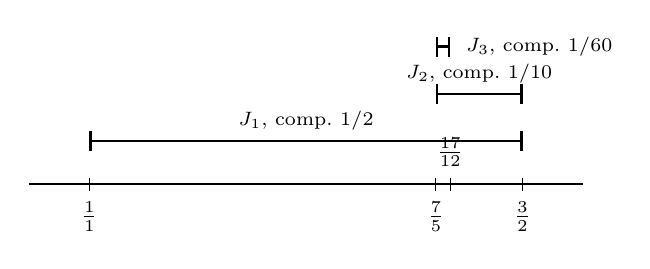
\begin{tikzpicture}[x=11cm,y=1cm]
  \draw[thick] (0.93,0) -- (1.57,0);
  \foreach \x in {1, 1.5, 1.4, 1.41667}{
    \draw (\x,0.08) -- (\x,-0.08);
  }
  \node[below] at (1,-0.1) {\small $\frac11$};
  \node[below] at (1.5,-0.1) {\small $\frac32$};
  \node[below] at (1.4,-0.1) {\small $\frac75$};
  \node[above] at (1.41667,0.1) {\small $\frac{17}{12}$};
  \draw[|-|,thick] (1,0.55) -- (1.5,0.55) node[midway,above]{\scriptsize $J_1$, comp.\ $1/2$};
  \draw[|-|,thick] (1.4,1.15) -- (1.5,1.15) node[midway,above]{\scriptsize $J_2$, comp.\ $1/10$};
  \draw[|-|,thick] (1.4,1.75) -- (1.41667,1.75) node[right,xshift=2pt]{\scriptsize $J_3$, comp.\ $1/60$};
\end{tikzpicture}
\end{center}

\begin{exemplo}
$\sqrt2 = \cf{1}{\overline{2}}$. A tabela abaixo é o produto $\Mat1\Mat2\Mat2\cdots$ lido coluna a coluna.
\begin{center}
\begin{tabular}{cccccc}
\toprule
$n$ & 0 & 1 & 2 & 3 & 4\\
\midrule
$p_n$ & 1 & 3 & 7 & 17 & 41\\
$q_n$ & 1 & 2 & 5 & 12 & 29\\
$p_n^2-2q_n^2$ & $-1$ & $1$ & $-1$ & $1$ & $-1$\\
\bottomrule
\end{tabular}
\end{center}
A última linha é o Corolário~\ref{cor:det} em ação (Pell), e $q_n/q_{n-1} = 12/5 = \cf{2}{2,2}$
ilustra o Teorema~\ref{thm:rev}.
\end{exemplo}

\subsection{O teorema de construção}

\begin{teorema}\label{thm:constr}
$(\Sig,\prec)$ é um conjunto totalmente ordenado, denso, sem extremos e \emph{completo}
(todo subconjunto não vazio limitado superiormente tem supremo). A aplicação
$\mathbf a \mapsto \bigcap_n J_n$ é um isomorfismo de ordem de $\Sig$ sobre $\R$, que leva as
palavras finitas em $\Q$ e as infinitas em $\R\setminus\Q$. Restrita às palavras infinitas, é
um homeomorfismo $\Z\times\Z_{\geq1}^{\N} \to \R\setminus\Q$ (o espaço de Baire).
\end{teorema}

\begin{proof}[Esboço]
Totalidade e densidade são imediatas da definição de $\prec$. Para a completude, dado
$S\subset\Sig$ não vazio e limitado, constrói-se o supremo \emph{letra a letra}: escolhe-se
$s_0 = \sup\{a_0 : \mathbf a \in S\}$ (finito pela limitação), depois, entre os elementos de $S$
que realizam $s_0$, escolhe-se $s_1$ como o \emph{ínfimo} dos $a_1$ (a orientação inverte),
e assim por diante; se o processo estaciona obtém-se uma palavra finita, senão uma infinita.
Verifica-se que a palavra resultante é cota superior e é $\preceq$ qualquer outra.
Que a aplicação para $\R$ é bem definida e injetiva é a Proposição~\ref{prop:encaixe} mais o
princípio dos intervalos encaixados; a sobrejetividade é o algoritmo da \S\ref{sec:revI}.
A afirmação topológica segue de que os cilindros $[a_0,\dots,a_n]$ são exatamente os traços dos
intervalos $J_n$ nos irracionais, e formam base de abertos com diâmetro $\to 0$.
\end{proof}

\begin{obs}[o preço e o prêmio]
Usar o Teorema~\ref{thm:constr} como \emph{definição} de $\R$ tem um preço, que é o das operações
de corpo, e um prémio. O preço está apurado na \S\ref{sec:condicoes}; é ele que faz de Dedekind e
Cauchy as construções de manual --- elas são \emph{aditivamente} naturais. O prémio é esta
construção trazer embutida a teoria da aproximação, que nas outras é um teorema à parte:
\[
  \left| x - \frac{p_n}{q_n}\right| < \frac{1}{q_nq_{n+1}} < \frac{1}{q_n^2},
\]
e os $p_n/q_n$ são as \emph{melhores} aproximações racionais no sentido forte.
\end{obs}

\begin{teorema}[Serret~\cite{serret} --- a construção é $\GL_2(\Z)$-equivariante]\label{thm:serret}
Dois irracionais $x,y$ têm palavras que coincidem a partir de certo índice se, e somente se,
$y = \gamma\cdot x$ para algum $\gamma\in\GL_2(\Z)$.
\end{teorema}

\noindent
Isto identifica o que a codificação realmente é: um sistema de coordenadas em $\Pj(\R)$ adaptado
à ação de $\GL_2(\Z)$. Trocar de palavra num prefixo finito $=$ agir por uma matriz inteira.

\subsection{As condições, reunidas}\label{sec:condicoes}

O que é preciso para dizer que a construção entrega $\R$ está espalhado por esta secção. Vale reuni-lo,
com o estatuto de cada peça declarado --- incluindo o que \emph{não} fica provado.

\begin{center}\small
\begin{tabular}{lll}
\hline
condição & onde & estatuto \\ \hline
ordem total & Teor.~\ref{thm:constr}, com a $\prec$ alternada & esboçado$^\dagger$ \\
densidade, sem extremos & Teor.~\ref{thm:constr} & esboçado \\
completude (supremo) & Teor.~\ref{thm:constr}, letra a letra & esboçado \\
\textbf{separabilidade} & as palavras finitas ($=\Q$), densas e numeráveis & \textbf{provado} \\
bijeção com $\R$ & Teor.~\ref{thm:constr} (intervalos encaixados) & esboçado \\
compatível com $\GL_2(\Z)$ & Teor.~\ref{thm:serret} & clássico, citado \\
topologia \emph{dos irracionais} & Teor.~\ref{thm:constr} (Baire $\cong\R\setminus\Q$) & esboçado \\[2pt]
\textbf{operações de corpo} & \S\ref{sec:constr} & \textbf{não sai das letras} \\
\hline
\end{tabular}
\end{center}

\noindent $^\dagger$ A prova do Teorema~\ref{thm:constr} é um \emph{esboço}, e a tabela di-lo:
numa secção cujo propósito é declarar estatutos, chamar ``provado'' ao que está esboçado seria o
erro que ela existe para evitar. Em particular a transitividade de $\prec$ é despachada com
``imediata da definição'' e exige análise de casos sobre o índice da primeira diferença.

A \textbf{separabilidade} entrou porque sem ela a caracterização não fecha: totalmente ordenado,
denso, sem extremos e completo \emph{não} caracteriza $\R$ --- a recta longa satisfaz os quatro e
não é isomorfa a $\R$. Falta o subconjunto denso numerável (Cantor), que aqui é de graça: são as
palavras finitas, isto é, $\Q$. E a linha da topologia diz \emph{dos irracionais} de propósito: o
que se obtém é o homeomorfismo com o espaço de Baire, que é totalmente desconexo, ao passo que
$\R$ é conexo --- é a Observação~\ref{obs:naosobe}.

Todas as linhas menos a última fecham (com o estatuto declarado) de dentro da construção. A última
não: \emph{não há fórmula razoável para as letras de $\mathbf a + \mathbf b$ em função das de
$\mathbf a$ e $\mathbf b$}. Define-se $+$ e $\cdot$ por continuidade a partir de $\Q$, ou pelo
algoritmo de Gosper --- que mantém um estado $2\times2\times2$, isto é, matrizes outra vez, mas já
não é o dicionário desta construção.

Portanto o enunciado exato do que se obtém é: \textbf{$(\Sig,\prec)$ é um conjunto totalmente
ordenado completo isomorfo a $\R$}, e não ``$\R$ como corpo ordenado completo''. A diferença não é
formalidade: o que caracteriza $\R$ a menos de isomorfismo é ser corpo ordenado completo, e a
estrutura de corpo entra aqui por fora. Dizer o contrário seria dar por fechada a única linha da
tabela que não fecha.

\begin{obs}[e o que \emph{não} está aqui]
Este texto não estabelece ligação entre a base assim construída e os zeros de $\zeta$. As duas
coisas tocam-se em vários pontos --- produto de Euler, Chebotarev, a fatoração de $\beta$ ---, mas
nenhuma dessas passagens está montada aqui como demonstração, e nenhuma o seria por analogia.
Registá-lo é preferível a insinuá-lo.
\end{obs}


\section{A realização hiperbólica}

\subsection{O lado par, e onde este texto entra}\label{sec:par}

A Observação~[I] deixou o lado $\det\rho(c)=+1$ como ``o que não vem de formas
holomorfas''. Dito assim parece um vazio; não é. É a outra metade, e tem objeto próprio:

\begin{center}\small
\begin{tabular}{lll}
\hline
 & $\det\rho(c)=-1$ (ímpar) & $\det\rho(c)=+1$ (par) \\ \hline
objeto automorfo & formas holomorfas & \textbf{formas de Maass} \\
peso & $k\geq1$ & $k=0$ \\
a equação & $\bar\partial f = 0$ (Cauchy--Riemann) & $\Delta f = \lambda f$ (Laplace) \\
o parâmetro & discreto (coeficientes de Fourier) & $\lambda = \tfrac14$ (isto é $r=0$) \\
\hline
\end{tabular}
\end{center}

\noindent \textbf{A coluna da direita é conjetural.} Que toda representação ímpar seja modular é
teorema (Wiles, e depois Khare--Wintenberger); que as \emph{pares} correspondam a formas de Maass
é conjectura --- de Maass, no quadro de Fontaine--Mazur ---, com só casos especiais estabelecidos.
Nada nesta tabela é deste texto, e a metade direita não é sequer conhecida. O que interessa aqui é que a ponte entre as duas colunas é a
\textbf{fórmula do traço de Selberg}~\cite{selberg1956}, e que o lado geométrico dessa fórmula é
uma soma sobre as \emph{geodésicas fechadas} de $\PSL_2(\Z)\backslash\Hyp$ --- que são, pelo
Teorema de Serret e por Series~\cite{series1985}, exatamente as fracções contínuas periódicas.

\begin{proposicao}[a família real é o lado geométrico]\label{prop:selberg}
Seja $A_m=\begin{psmallmatrix}m&1\\1&0\end{psmallmatrix}$, de autovalor dominante
$\sigma = (m+\sqrt{m^2+4})/2$ --- a raiz de $\beta_{2,m}$. Como $\det A_m = -1$, a classe que
representa uma geodésica fechada de $\PSL_2(\Z)\backslash\Hyp$ é a de $A_m^2$ (traço $m^2+2$,
autovalor $\sigma^2$), e o comprimento é
\[
  \ell_m \;=\; 2\log(\sigma^2) \;=\; 4\log\sigma .
\]
\end{proposicao}

\begin{proof}
Uma classe hiperbólica de $\SL_2(\Z)$ de autovalor dominante $\lambda>1$ dá geodésica fechada de
comprimento $2\log\lambda$. Ora $A_m \notin \SL_2(\Z)$: $\det A_m = -1$, logo $A_m$ vive em
$\GL_2(\Z)$ e não representa classe em $\PSL_2(\Z)$. A menor potência com determinante $+1$ é
$A_m^2$, de autovalor $\sigma^2$. Equivalentemente, em termos de unidades: $N(\sigma) = -1$, e o
comprimento é $2\log\varepsilon$ com $\varepsilon$ a unidade fundamental de \emph{norma $+1$}, que
aqui é $\sigma^2$.
\end{proof}

\noindent Para $m=1,2,3,5,7$: $\ell = 1{,}924847;\ 3{,}525494;\ 4{,}779053;\ 6{,}588925;\
7{,}862882$. O primeiro valor é um controlo útil: $4\log\varphi = 1{,}9248\ldots$ é o comprimento
da \emph{geodésica mais curta} da superfície modular, número clássico --- e é o que dá a fracção
contínua $\overline{1}$, a mais simples de todas. (Tomar $2\log\sigma$ daria metade disso e não
bateria com o valor conhecido: o determinante $-1$ não é detalhe de arrumação.)

Ou seja: o $\sigma$ deste texto \emph{é} o autovalor da classe hiperbólica, a sua fracção contínua
$\overline{m}$ \emph{é} a geodésica, e o lado geométrico de Selberg é uma soma sobre unidades de
Pell. Somar sobre reguladores de um lado e sobre autovalores do Laplaciano do outro é a mesma soma
vista pelas duas caras. A analogia certa não é a dualidade de Pontryagin --- essa é para grupos
localmente compactos \emph{abelianos} --- mas a soma de Poisson, de que a fórmula do traço é o
análogo não-abeliano.

\begin{obs}[e o sinal, outra vez]
$\det A_m = -1$. A involução que troca $\sigma$ por $1/\sigma$ vem com sinal negativo, e é o mesmo
$-1$ que aparece em $\det\rho(c)$ do lado de Galois. Nos dois sítios é o sinal que impede o par de
colapsar num ponto: sem ele a involução seria a identidade e não haveria dois lados para trocar.
\end{obs}


\section{O par aditivo e o multiplicativo}\label{sec:aditmult}

As duas famílias de progressões --- a de razão fixa e a de passo fixo --- são as duas faces
da mesma coisa, e $\exp$ é o que as troca. Esta secção estabelece-o e apura o que a figura
não suporta.

\begin{proposicao}[P.A. e P.G. são duais: $\exp$ conjuga as duas involuções]\label{prop:conjuga}
Cada lado tem uma involução natural, e é a única \emph{contínua} que a sua operação admite:
\[
  \nu_+(r) = -r \quad\text{(negar, do lado aditivo)}, \qquad
  \nu_\times(q) = 1/q \quad\text{(inverter, do lado multiplicativo)} .
\]
E são a \emph{mesma} involução, conjugada por $\exp$:
\[
  \nu_\times \circ \exp \;=\; \exp \circ\, \nu_+ ,
\]
isto é, $e^{-r} = 1/e^{r}$. Os pontos fixos correspondem-se pela mesma conjugação:
$\nu_+$ fixa $r=0$, $\exp(0)=1$, e $\nu_\times$ fixa $q=1$.
\end{proposicao}

\noindent Convém ser exato sobre o que é de $\exp$ e o que não é. A relação $f(-r) = 1/f(r)$
\textbf{não} caracteriza $\exp$: vale para todo $f = e^{g}$ com $g$ ímpar (por exemplo
$e^{r^3}$), e até para a Möbius $f(r) = \frac{1+r}{1-r}$, que nem exponencial é. Falha, isso sim,
para $f(x)=x+1$, $f(x)=x^2+1$ e $f = e^{r^2}$.

O que $\exp$ tem de único é outra coisa, e é essa que importa: é o \textbf{único homomorfismo
contínuo} $(\R,+) \to (\R_{>0},\times)$ a menos de escala. Conjugar a involução é consequência
disso, não o contrário. E é isto que dá sentido preciso a ``a P.A. é a sombra da P.G.'': a P.A.
\emph{é} a P.G. lida em logaritmo, onde inverter vira negar.

A ressalva já conhecida encaixa aqui: $\nu_\times$ fixa também $q=-1$, e esse ponto fixo não tem
imagem real por $\exp$ --- $\log(-1) = i\pi$ está fora do eixo. É a razão estrutural de $q=-1$ não
dar a P.A. (Prop.~\ref{prop:papg}).



\begin{obs}[a P.A. de ordem $m$ é a fronteira]\label{obs:pam}
A progressão aritmética de ordem $m$ é definida pela recorrência $a_{n,m} = a_{n-1,m} +
a_{n-1,m-1}$, cuja matriz é triangular com $1$ na diagonal: \textbf{unipotente}, todos os
autovalores iguais a $1$. Unipotente é a generalização de ``parabólica'' para dimensão maior que
$2$ (o critério do traço só se enuncia em $\SL_2$). Uma P.A. não expande nem roda: \emph{translada}
--- e é por isso que fica exatamente na fronteira entre as outras duas classes.

A P.G. de ordem $m$ é a mesma escada com razão $q$, de autovalores $1,q,\dots,q^m$: hiperbólica se
$q$ é real $\neq1$, elíptica se $|q|=1$. A conversão P.A.$_m \leftrightarrow$ P.G.$_m$ é
$\exp/\log$, e é ela que troca uma classe pela outra, porque leva ``somar $r$'' em ``multiplicar
por $e^r$''. \emph{O logaritmo é o que converte translação em expansão} --- é também ele que
aparece no comprimento $\ell = 4\log\sigma$ da Proposição [II].
\end{obs}

\begin{proposicao}[P.A. e P.G. são duais por $\nu$, e a P.A. é o ponto fixo]\label{prop:papg}
A involução $\nu\colon \lambda\mapsto1/\lambda$ age nas razões e leva
$\mathrm{P.G.}_m(q)$ em $\mathrm{P.G.}_m(1/q)$: os espectros $\{q^k\}$ e $\{q^{-k}\}$ trocam-se
termo a termo. O conjunto \textbf{fixo} é $q = 1/q$, isto é $q\in\{+1,-1\}$; em $q=+1$ a P.G.
degenera exatamente na P.A.$_m$ do Gentil.
\end{proposicao}

\noindent A degenerescência é a colisão dos autovalores. Se $q$ \emph{não} é raiz da unidade de
ordem $\leq m$, os $m+1$ valores $1,q,\dots,q^m$ são distintos, a matriz é diagonalizável e há
$m+1$ direções próprias. Em $q=+1$ colidem todas, a matriz passa a bloco de Jordan --- literalmente
a de $a_{n,m}=a_{n-1,m}+a_{n-1,m-1}$ ---, e o espaço próprio cai para $\mathbf 1$. (A ressalva é
necessária: em $m=2$, $q=-1$, o espectro é $\{1,1,-1\}$ e há $2$ direções, nem $m+1$ nem $1$ --- o
outro ponto fixo da involução não dá a P.A.)

\begin{center}\small
\begin{tabular}{cccc}
\hline
$m$ & direções da P.G.$_m$ ($q$ genérico) & da P.A.$_m$ & perdidas \\ \hline
$1$ & $2$ & $1$ & $1$ \\
$2$ & $3$ & $1$ & $2$ \\
$3$ & $4$ & $1$ & $3$ \\
$4$ & $5$ & $1$ & $4$ \\
\hline
\end{tabular}
\end{center}

\noindent \textbf{A P.A.$_m$ é a sombra da P.G.$_m$}: as $m+1$ direções que na dimensão de cima se
separam ficam reduzidas a uma só direção própria, e o resto do movimento passa a nilpotente --- a
translação. Convém ser exato sobre o que cai: o espaço de \emph{soluções} continua com dimensão
$m+1$ (passa a ser o dos polinómios de grau $\leq m$ em $n$); o que colapsa é o espaço
\emph{próprio}. E a colisão de autovalores é necessária mas não suficiente para isso --- a
identidade tem-nos todos colididos e é diagonal; aqui a estrutura de Jordan vem da forma da
recorrência, não só da colisão.

Gentil escreve que a transformação leva ``uma P.A. de ordem $k$ numa P.G. de ordem $k$ e
reciprocamente''. Isso é exato \emph{fora} do ponto fixo; sobre ele a correspondência deixa de ser
bijeção, porque o logaritmo colapsa. E é precisamente aí --- em $|\lambda|=1$, onde $\nu$ fixa ---
que reaparece tudo o resto: os pontos fixos da involução (Obs. (I1)), a raiz de
$\beta_{5,1}$ que estraga a matriz (Prop. (I7)) e a ramificação de $p=2$ em $\Z[i]$.
\emph{A fronteira é uma só, e é sempre a mesma: o lugar onde a involução tem ponto fixo.}


\paragraph{A razão da P.A. é o metal.} A recorrência da Proposição (I4) em $n=2$ é
$t_k = m\,t_{k-1} + t_{k-2}$: a P.A. de \textbf{razão $m$}. Percorrendo $m = 1,2,3,4,\dots$
percorrem-se as famílias metálicas, uma por razão --- e a ligação entre o inteiro e o irracional é
a involução:
\[
  \sigma_m + \sigma'_m \;=\; m \quad(\text{o traço}), \qquad
  \sigma_m \cdot \sigma'_m \;=\; -1 \quad(\text{o determinante}),
  \qquad \sigma'_m = -1/\sigma_m .
\]

\begin{center}\small
\begin{tabular}{clll}
\hline
$m$ & metal & $\sigma_m = (m+\sqrt{m^2+4})/2$ & a P.A. inteira $t_k$ \\ \hline
$1$ & ouro ($\varphi$) & $1{,}6180339887$ & $1,3,4,7,11,18,\dots$ (Lucas) \\
$2$ & prata & $2{,}4142135624$ & $2,6,14,34,82,\dots$ \\
$3$ & bronze & $3{,}3027756377$ & $3,11,36,119,393,\dots$ \\
$4$ & --- & $4{,}2360679775$ & $4,18,76,322,1364,\dots$ \\
$5$ & --- & $5{,}1925824036$ & $5,27,140,727,3775,\dots$ \\
\hline
\end{tabular}
\end{center}

\noindent \emph{E o circuito fecha, reversível em cada passo.} Parte-se do inteiro $m$; a
companheira dá $A_m$; o autovalor dá o irracional $\sigma_m$; a conjugação dá $\sigma'_m$
(Obs. (I3) --- é a conjugação e não $\nu$, pelo sinal); a soma devolve $m$. Sem perda
e sem aproximação:
\[
  m \;\longmapsto\; A_m=\Mat{m} \;\longmapsto\; \sigma_m \;\longmapsto\;
  \sigma'_m = -1/\sigma_m \;\longmapsto\; \sigma_m + \sigma'_m \;=\; m .
\]
O que torna o percurso exato é a fórmula de \textbf{Vieta}: num mónico $x^2-mx+c$ as raízes somam
$m$, seja qual for $c$. Não é o determinante --- $x^2-5x-7$ tem $\det = -7$ e as raízes somam $5$
na mesma. O que $|\det|=1$ dá, e é outra coisa, é que o \emph{segundo} autovalor seja $-1/\sigma$:
sem essa condição há circuito de igual modo, mas não há involução recíproca. Nesse sentido o
circuito é circular de maneira inócua --- $m$ entra como traço e é recuperado como traço --- e o
que se ganha não é a volta em si, mas o facto de o caminho de regresso ser a conjugação.

\begin{obs}[$K_{n,m}$ \emph{não} é a P.A. de ordem $n$ e razão $m$ --- e o que os separa é a classe]\label{obs:naopa}
A tentação é natural: os dois objetos têm dois parâmetros, e um deles chama-se ordem. Mas a
comparação faz-se pelo polinómio característico, e aí eles nunca coincidem:
\[
  \mathrm{P.A.}_m \;\rightsquigarrow\; (x-1)^{m+1},
  \qquad
  K_{n,m} \;\rightsquigarrow\; x^n - m\,x^{n-1} - 1 .
\]
O primeiro tem todas as raízes em $1$; o segundo nunca tem $1$ por raiz, porque
$\beta_{n,m}(1) = -m \neq 0$. Um é unipotente, o outro é de Pisot --- parabólico contra hiperbólico,
a dicotomia da \S(I7).

E os \emph{papéis} dos parâmetros também diferem. Na P.A. do Gentil a razão $r$ é uma
\textbf{condição inicial} ($a_{n,0}=r$): mudá-la escala a sequência e \emph{não mexe no espectro} ---
por isso a P.A. permanece parabólica seja qual for a razão. Em $K_{n,m}$, o $m$ é um
\textbf{coeficiente} da recorrência: é ele que move $\sigma$. Não são o mesmo $m$.

\begin{obs}[e uma tentação a evitar: normalizar não é medir]\label{obs:pu}
É tentador dizer que $m$ não é um eixo genuíno mas apenas a \emph{unidade} da reta, e sustentá-lo
observando que ``em p.u.'' a razão vale $1$ para todo $m$:
$\sigma_m^{-1}\lim_k t_{k+1}/t_k = 1$ e $(\sigma+\sigma')/m = 1$. \textbf{Nenhuma das duas mede
coisa alguma}: são a mesma quantidade dividida por si própria, e dariam $1$ para qualquer
sequência. Uma verificação que não pode falhar não é verificação.

Pior, o ``colapso'' que elas sugeririam é falso. Normalizar uma matriz é multiplicá-la por um
escalar $c$, e isso leva $(\operatorname{tr},\det) = (m,-1)$ em $(cm,-c^2)$: impor $cm=1$ força
$c = 1/m$ e dá $\det = -1/m^2$, que vale $-1$ \emph{só} em $m=1$ ($-\tfrac14$ para $m=2$,
$-\tfrac19$ para $m=3$). Não existe escala que torne todos os metais na mesma matriz --- pelo
contrário, $\Comp{2}{m}/m$ degenera para uma matriz \textbf{singular}. O que se passava era que as
duas ``normalizações'' eram diferentes: o traço dividido por $m$ e o determinante dividido por
nada.

O que \emph{é} verdade, e sem p.u. nenhum, é o parágrafo anterior: na P.A. do Gentil a razão é
condição inicial e não move o espectro; em $K_{n,m}$ o $m$ é coeficiente e move $\sigma$. Isso
sustenta-se sozinho. E há um facto na direção contrária que convém não esconder: $\sigma_{n,m} \to
m$ quando $n$ cresce (para $m=3$: $3{,}303$; $3{,}104$; $3{,}012$; $3{,}000051$), isto é, subir de
dimensão faz o irracional convergir para o inteiro $m$ --- o que argumenta que $m$ é precisamente
o que \emph{fica}, não o que se pode normalizar para fora.
\end{obs}

\emph{O que é verdade} é mais interessante do que a identificação falsa: as duas são recorrências
lineares de ordem $n$, e ocupam os dois \textbf{extremos} da mesma família. A P.A. é o caso em que
todos os autovalores colidem em $1$ (Prop.~\ref{prop:papg}); $K_{n,m}$
é o caso em que um escapa para fora e os outros ficam dentro. Entre os dois está tudo o resto.

A sequência que de facto pertence a $K_{n,m}$ é a da Proposição (I4),
$t_k = m\,t_{k-1} + t_{k-n}$: aí sim a \emph{ordem} é $n$ e o \emph{coeficiente} é $m$, e a P.A.
do Gentil é o que ela se torna quando o espectro colapsa.
\end{obs}


\section{As duas coordenadas}\label{sec:coord}

\subsection{As duas como coordenadas da recta}\label{sec:duascoord}

Sendo duais, elas não competem: \textbf{coordenam}. Fixada uma razão $q>1$, todo $x>0$ escreve-se
de uma só maneira como
\[
  x \;=\; q^{\,k+\theta}, \qquad k\in\Z \ \text{(a P.G.)}, \qquad \theta\in[0,1) \ \text{(a P.A.)} .
\]
A P.G. dá o \emph{passo} --- a órbita $\dots,q^{-1},1,q,q^2,\dots$ --- e a P.A. dá a posição
\emph{dentro} do passo. Uma conta, a outra mede.

\begin{proposicao}[cobertura sem buraco e sem sobreposição]\label{prop:coord}
$x \mapsto (k,\theta)$ é uma bijeção \emph{de conjuntos} de $\R_{>0}$ sobre $\Z\times[0,1)$, e com
o sinal, de $\R\setminus\{0\}$ sobre $\{\pm1\}\times\Z\times[0,1)$.
\end{proposicao}

\noindent \textbf{De conjuntos, e só.} Não há homeomorfismo: $\Z\times[0,1)$ com a topologia
produto é desconexo --- cada $\{k\}\times[0,1)$ é aberto e fechado --- ao passo que $\R_{>0}$ é
conexo. É exatamente o mesmo cuidado da Observação~(I6), e não custa repeti-lo: uma
bijeção que reorganiza não é uma identificação que preserve estrutura.

\noindent A bijeção prova-se em duas linhas: $k = \lfloor \log_q x\rfloor$ e
$\theta = \log_q x - k$ definem a inversa, e a unicidade é a da parte inteira. Corremos também
$200\,000$ pontos com erro relativo máximo $5{,}2\times10^{-16}$, mas convém dizer o que isso mede:
é o \emph{epsilon} da implementação de $\exp/\log$, não a bijeção. (E que $\theta$ saia uniforme é
automático, porque a amostra foi log-uniforme --- mediria a convenção de amostragem, não o objeto.)

A \textbf{vírgula flutuante} tem a mesma forma --- sinal, expoente, resto --- mas \emph{não} é a
mesma decomposição, e vale corrigi-lo antes que a semelhança engane. Nela escreve-se $x = m\cdot2^e$
com a mantissa $m\in[1,2)$ \textbf{linear} e finita (52 bits em binário64); aqui escreve-se
$x = 2^{k+\theta}$ com $\theta$ \textbf{logarítmico} e real. As duas relacionam-se por
$m = 2^{\theta}$ --- que é precisamente a conjugação da Proposição~\ref{prop:conjuga}. Dizer que
``é a mesma conta'' seria dizê-lo \emph{a menos de $\exp$}, e $\exp$ é justamente o objeto em
disputa.

O zero fica de fora por necessidade, porque $\log 0 = -\infty$: é exatamente o ponto que a Möbius
$J(z)=1/z$ manda ao infinito, o único que nenhuma das duas coordenadas alcança, e por isso é ele
que fecha a esfera.


\subsection{A zeta de Riemann na mesma linguagem}\label{sec:zetariemann}

A \S(I4) exibiu uma zeta \emph{dinâmica}, racional. A de Riemann encaixa na mesma
gramática, e vale escrevê-lo --- com o cuidado de dizer, no fim, o que isso não dá.

\paragraph{A P.A. de razão $1$, dualizada termo a termo.} A P.A. de razão $1$ é $1,2,3,\dots$ ---
os naturais, o índice puro. Dualizando cada termo pela conjugação da Proposição~\ref{prop:conjuga},
$n \mapsto n^{-s} = \exp(-s\log n)$, e somando:
\[
  \zeta(s) \;=\; \sum_{n\,\in\,\mathrm{P.A.}(1)} \exp(-s\log n) ,
\]
tudo para $\operatorname{Re}(s) > 1$, onde a série converge absolutamente. E o \textbf{produto de
Euler} tem do outro lado uma P.G. por primo, $(1-p^{-s})^{-1} = 1 + p^{-s} + p^{-2s} + \cdots$:
\[
  \sum_{n\geq1} n^{-s} \;=\; \prod_p (1-p^{-s})^{-1} \qquad (\operatorname{Re}(s)>1) .
\]
\emph{A fatoração única e o produto de Euler são o mesmo enunciado}, e vale dizer pelo mecanismo
certo: expandindo o produto pela distributiva, cada $n$ aparece \textbf{exatamente uma vez} ---
pelo menos uma pela existência da fatoração, no máximo uma pela unicidade ---, e a convergência
absoluta é o que autoriza o rearranjo. \textbf{A conjugação $\exp/\log$ não entra em passo nenhum
disto}, e seria erro atribuir-lho: Euler usa só a estrutura multiplicativa de $\N$, e a soma de
índices nunca aparece.

E são \emph{os primos}, não outro conjunto: com todos os inteiros $\geq2$ o produto dá $2$
exatamente ($\prod_{n\geq2}(1-n^{-2})^{-1}=2$) e pelos ímpares dá $4/\pi = 1{,}2732$, contra
$\zeta(2) = \pi^2/6$.

\paragraph{Parte real e parte imaginária: P.G. e P.A.} Escrevendo $s = a+it$,
\[
  n^{-s} \;=\; \underbrace{n^{-a}}_{\text{módulo}} \cdot
               \underbrace{\exp(-it\log n)}_{\text{fase}} .
\]
Ao dobrar $n$, o módulo \emph{multiplica} por $2^{-a}$ e o argumento \emph{soma} $-t\log 2$: a parte
real gera uma P.G. (razão $2^{-a}$ por duplicação de $n$), a imaginária uma P.A. (passo
$-t\log2$). E ``dá no mesmo'' tem sentido exato --- lidas em logaritmo, \emph{ambas} são P.A., de
passos $-a$ e $-t$ por unidade de $\log n$; é o $\exp$ que veste uma de multiplicativa e deixa a
outra aditiva. Reencontra-se aqui o sinal de sempre: a parte real é hiperbólica
($\cosh/\senh$, expande), a imaginária elíptica ($\cos/\sen$, roda).

\begin{obs}[$\operatorname{Re}(s)=\tfrac12$ é o conjunto fixo de $s\mapsto1-\bar s$ --- um facto sobre a aplicação, não sobre $\zeta$]\label{obs:critica}
Fora do semiplano acima, $\zeta$ define-se por continuação meromorfa, e aí valem \textbf{duas}
simetrias, de proveniências distintas --- convém não as colar:
\begin{itemize}\itemsep2pt
\item a \emph{equação funcional}, $\xi(s) = \xi(1-s)$, que dá a involução $w(s) = 1-s$;
\item o \emph{princípio de reflexão de Schwarz}, $\zeta(\bar s) = \overline{\zeta(s)}$, que dá a
involução $c(s) = \bar s$. Este é facto independente, não parte da equação funcional.
\end{itemize}
Só a \textbf{composta} $w\circ c\colon s\mapsto 1-\bar s$ tem por conjunto fixo a recta
$\operatorname{Re}(s)=\tfrac12$. E o trabalho é quase todo da conjugação: $w$ sozinha fixa apenas
o \emph{ponto} $s=\tfrac12$; $c$ sozinha fixa o eixo real. (As quatro aplicações formam o
quadrigrupo de Klein $\{\mathrm{id},\,1-s,\,\bar s,\,1-\bar s\}$.)

O conjunto fixo não sai de ``ser involução'' --- isso não determina nada, como mostram os três
exemplos acima, com fixos de dimensão $1$, $1$ e $0$. Sai de \emph{resolver} $s = 1-\bar s$: com
$s = \sigma+it$ vem $\sigma = 1-\sigma$, logo $\sigma=\tfrac12$ e $t$ livre.

\textbf{E aqui o padrão da casa não morde --- é o que interessa dizer.} Nas outras instâncias deste
texto, ``a fronteira é onde a involução tem ponto fixo'' \emph{explica} algo do objeto: porque
$\beta_{5,1}$ falha, porque $p=2$ ramifica, porque $q=1$ degenera. Aqui não explica nada sobre
$\zeta$, e a razão é exata: \emph{o conjunto fixo de $s\mapsto1-\bar s$ é
$\operatorname{Re}(s)=\tfrac12$ quer $\zeta$ exista quer não} --- é o mesmo para qualquer função
com a mesma equação funcional, e seria o mesmo se $\zeta$ não existisse. É um facto sobre a
\emph{aplicação}, não sobre a função.

O que de facto se segue é uma \emph{simetria}: se $\rho$ é zero, $1-\bar\rho$ também. Que os zeros
\emph{estejam} sobre a recta é a Hipótese de Riemann, está em aberto, e nada nesta secção a toca
nem se aproxima dela. Simetria não é localização --- a mesma distinção que o
Corolário~(I2) obriga a fazer noutro contexto: uma condição que os zeros satisfazem
não é uma condição que os localize.
\end{obs}


\subsection{As duas no tempo: a espiral, o cone, o hipercubo}\label{sec:dinamica}

Deixando o tempo correr nas duas coordenadas ao mesmo passo --- a P.G. no raio, a P.A. no ângulo ---
\[
  r(t) = q^{\,t}, \qquad \alpha(t) = t\cdot\omega ,
\]
obtém-se a \textbf{espiral logarítmica}. A sua assinatura é a de as duas correrem juntas: o ângulo
entre o raio e a tangente é \emph{constante} em todo o ponto (por isso se lhe chama
\emph{equiangular}). Para $q=\varphi$ e $\omega = 2\pi/\varphi$ esse ângulo vale $82{,}9359^\circ$,
igual em $\alpha = 0{,}5$, $3$ ou $10$, e a razão entre raios sucessivos é sempre $\varphi$.

\paragraph{O cone é recto no eixo logarítmico.} Juntando a altura como o tempo puro, a razão
$r/h$ \textbf{não} é constante --- $1{,}618$; $1{,}309$; $1{,}412$; $1{,}714$; $2{,}218$ para
$t=1,\dots,5$ ---, logo não é cone recto no sentido usual. Mas $\log r / h$ é constante e vale
$\log\varphi = 0{,}481211825$ em todos. \emph{O cone é recto onde a P.G. vira P.A.}, e a espiral é
a sua projeção --- o que dá conteúdo à figura cone/espiral usada informalmente noutros pontos.

\paragraph{E em dimensão $n$, o hipercubo é a célula.} Aplicando as duas coordenadas a cada
entrada de $\R_{>0}^n$, o expoente vive em $\Z^n$ e o resto em $[0,1)^n$: \textbf{o hipercubo
semiaberto é a célula fundamental do reticulado}, e as suas cópias ladrilham $\R_{>0}^n$ sem buraco
e sem sobreposição. Verificado para $n=2,3,4$ com $40\,000$ pontos cada: $100\%$ dos restos caem em
$[0,1)^n$ e o erro máximo de reconstrução é $5{,}6\times10^{-16}$.

Aqui a ressalva da \S\ref{sec:duascoord} melhora em vez de piorar. É verdade que
$\Z^n\times[0,1)^n$ com a topologia produto é desconexo e $\R_{>0}^n$ não é; mas o objeto
geométrico certo não é o produto --- é o \textbf{quociente} $\R^n/\Z^n$, o \emph{toro}, que é
conexo e compacto. Ladrilhar com o hipercubo e passar ao toro são a mesma operação vista por dentro
e por fora, e é a estrutura de \emph{reticulado} que sobrevive --- a mesma que aparece no mergulho
de Minkowski da \S[I].

\begin{obs}[nada real fica no ponto fixo, e é o desvio que codifica]\label{obs:desvio}
A observação anterior tem um complemento que vale registar, e que é geral: \emph{o ponto fixo de
uma involução é o lugar de menor informação}. Se tudo estivesse exatamente sobre ele não haveria
nada a codificar --- o ponto fixo sozinho é \textbf{um} número, e é a sequência de desvios que
separa os infinitos irracionais.

Mede-se na própria régua deste texto. A palavra de $\varphi$ é $\overline{1}$, e a sua entropia por
letra é \textbf{zero}: não carrega informação nenhuma além de si própria. Para $\sqrt2 =
[1;\overline{2}]$ é $0{,}169$ bits, e para $\pi$ é $2{,}92$. E os convergentes nunca chegam:
$|\varphi - p_n/q_n|$ decresce mas não se anula, com $q_n^2|\varphi-p_n/q_n| \to 1/\sqrt5$ --- o
desvio \emph{tem lei}, e é a lei que distingue.

Isto explica, aliás, a aparente contradição do Teorema de Hurwitz (\S[I]): $\varphi$ é
ao mesmo tempo o irracional de \emph{palavra mais simples} e o \emph{mais difícil de aproximar}, e
as duas coisas são a mesma. Entropia zero é a cristalização perfeita; a constante $1/\sqrt5$ é o
preço que ela cobra. Qualquer realização finita fica \emph{perto} do ponto fixo e não nele, e é
precisamente essa diferença que constitui a assinatura --- $e$, $\pi$ e $\sqrt2$ convergem todos,
e o que os distingue não é para onde vão mas \emph{como se desviam pelo caminho}.
\end{obs}


\section{A roupa da zeta}\label{sec:zetacap}

\subsection{As mesmas operações na roupa da zeta}\label{sec:zetaelastica}

A \S\ref{sec:operacoes} fez adição, multiplicação e ordem por reordenação de uma série geométrica.
A zeta admite o mesmo tratamento --- e o exercício vale sobretudo pelo que \emph{não} atravessa.

\paragraph{Soma: partição em P.A.} Partindo os índices em classes de resto módulo $r$,
\[
  \zeta(s) \;=\; \sum_{i=1}^{r} \ \sum_{n\equiv i \,(r)} n^{-s} ,
\]
e a soma das classes devolve o total, para todo $r$ (verificado para $r=2,3,5,7$ com resíduo nulo).
É a decomposição clássica em progressões aritméticas --- cada classe é, a menos de caracteres, uma
$L$-função de Dirichlet. \emph{A massa conserva-se}: é o elástico da \S\ref{sec:operacoes}, na
mesma forma.

\paragraph{Multiplicação: P.G. por primo.} É o produto de Euler, já visto: cada fator
$(1-p^{-s})^{-1}$ é uma P.G. de razão $p^{-s}$.

\paragraph{E o elástico não tem uma fronteira: tem quatro.} Convém separar dois factos que se
sobrepõem no mesmo plano.

\emph{Primeiro, a convergência.} Reordenar só é operação livre onde ela é absoluta:

\begin{center}\small
\begin{tabular}{lll}
\hline
regime & reordenar & o elástico \\ \hline
$\operatorname{Re}(s)>1$ & não muda o valor & \textbf{rígido} \\
$\operatorname{Re}(s)\leq1$ & muda o valor & \textbf{estica} \\
\hline
\end{tabular}
\end{center}

\noindent Medido: em $s=2$ e $s=1{,}5$ uma permutação aleatória de $60\,000$ termos devolve o mesmo
valor ao último bit. Já na série alternada, que converge condicionalmente para $0<s\leq1$,
reordená-la dois positivos por cada negativo leva $0{,}6931$ a $1{,}0397$ em $s=1$, e $0{,}6423$ a
$12{,}82$ em $s=0{,}7$ --- é o teorema do rearranjo de Riemann. \emph{Fora do semiplano de
convergência absoluta, mudar a ordem não é reorganizar o mesmo objeto: é trocar de objeto.} E a
recta crítica está do lado elástico. Note-se que $\operatorname{Re}(s)>1$ e
$\operatorname{Re}(s)<0$ são \emph{imagem um do outro} por $w(s)=1-s$: são o mesmo lado, visto
pelos dois lados, e a faixa crítica é o que sobra entre eles.

\emph{Segundo, e independente: a simetria parte o plano em quatro.} As duas involuções da
Observação~\ref{obs:critica} --- $w(s)=1-s$ e $c(s)=\bar s$ --- geram o quadrigrupo de Klein
$\{\mathrm{id},w,c,wc\}$, verificado: cada elemento é o seu próprio inverso e o produto de dois
distintos dá o terceiro. A órbita de um ponto genérico tem \textbf{quatro} elementos, e as
``fronteiras'' são exatamente os lugares onde ela \emph{encolhe}:

\begin{center}\small
\begin{tabular}{lll}
\hline
onde & órbita & o que a fixa \\ \hline
genérico ($0{,}37+1{,}9i$) & $4$ pontos & só a identidade \\
sobre $\operatorname{Re}(s)=\tfrac12$ & $2$ pontos & $wc$ \\
sobre o eixo real & $2$ pontos & $c$ \\
em $s=\tfrac12$ & $1$ ponto & tudo \\
\hline
\end{tabular}
\end{center}

\noindent \emph{Não há uma fronteira e um interior: há uma estratificação por estabilizadores}, e
os quatro estratos são os quatro duais. É a mesma figura da \S(I7) --- elíptico,
parabólico, hiperbólico separados pelo que a involução fixa --- agora com o grupo completo à vista
em vez de uma involução isolada.

\begin{obs}[e as outras duas não atravessam]\label{obs:naoatravessa}
Convém dizer onde a analogia para, para não a esticar também.

\textbf{Ordem:} existe no eixo real, e por razão elementar --- $n^{-a}>n^{-b}$ para $n\geq2$ e
$a<b$, logo $\zeta$ é estritamente decrescente em $s>1$ ($2{,}6087 > 1{,}6449 > 1{,}2021 >
1{,}0823$). Mas \emph{não} há ordem no plano, e a razão é directa: $-1 = i^2$, logo $\C$ não é formalmente
real e Artin--Schreier exclui-o sem ser preciso invocar $r_1$ (que nem está definido para $\C$, que
não é corpo de números). A ordem alternada deste texto é da recta, e não sobe.

\textbf{Completude:} não atravessa, mas não pela razão que primeiro ocorre. Dizer que os valores
``não são fechados'' é \emph{falso}: $\zeta$ é contínua e estritamente decrescente em $s>1$, com
$\zeta(1^+)=+\infty$ e $\zeta(\infty)=1$, donde $\zeta((1,\infty)) = (1,\infty)$ exatamente --- e
esse conjunto \emph{é} fechado para $+$ e $\times$. Só que lhe faltam $0$, $1$, simétricos e
inversos: é semianel, não corpo. E no domínio completo a imagem de $\zeta$ é $\C$ (Landau; ou
Picard, por $\infty$ ser singularidade essencial), pelo que ``os valores formam um corpo'' passa a
verdade \emph{vazia} --- o corpo é $\C$, $\zeta$ não contribuiu com nada, e $\C$ não é ordenável.
(Invocar a transcendência de $\pi^2/6$ não serviria: $\R$ está cheio de transcendentes e é corpo.)

Das quatro condições, portanto, \textbf{duas atravessam} (soma e multiplicação, por reordenação),
\textbf{uma atravessa em parte} (ordem, só no eixo real) e \textbf{uma não atravessa}
(completude). É um resultado melhor do que se atravessassem as quatro: onde a analogia falha é
onde ela estava a ser usada como argumento em vez de como figura.
\end{obs}


\section{As áreas}\label{sec:areascap}

\subsection{As áreas são as coordenadas}\label{sec:areas}

A \S\ref{sec:duascoord} tomou como coordenadas o expoente e o resto. Há um par melhor, e é o que
torna a construção reversível: as \textbf{áreas}. Percorrida a curva de Hilbert até ao índice $d$
de $N$ células, a área \emph{branca} --- o que já foi codificado --- vale $d/N$, e a \emph{negra}
--- o que falta --- vale $1-d/N$. Elas somam $1$, exatamente, em todo ponto do percurso: é o
elástico da \S\ref{sec:operacoes} na sua forma mais simples, com uma coordenada a ser o complemento
da outra.

\begin{proposicao}[o processo é único e reversível]\label{prop:areas}
Em cada nível finito (lado $2^p$, células discretas), $d \mapsto (x,y)$ é uma bijeção e a área
branca determina a célula. A reversão do percurso, $d\mapsto N-1-d$, é involução exata sobre
índices e troca branca com negra \emph{a menos de uma célula}: $\text{branca}(N-1-d) =
\text{negra}(d) - 1/N$.
\end{proposicao}

\noindent Verificado para lado $32$: os $1024$ índices fazem $d\to(x,y)\to d$ sem uma falha. O
desvio de $1/N$ na troca das áreas é exato e não de arredondamento; vai a zero no refinamento, mas
enquanto se está num nível finito ele está lá. \emph{No limite a bijeção não sobrevive}: a curva de
Hilbert é sobrejeção contínua $[0,1]\to[0,1]^2$ e não é injetiva --- tem de não ser, porque $[0,1]$
e $[0,1]^2$ não são homeomorfos (Obs.~(I6)).

\paragraph{E o refinamento conserva.} A fracção branca num mesmo ponto relativo é \emph{invariante}
por refinamento --- vale $1/4$ em $d=N/4$ para lado $4,8,16,\dots,256$, ao dígito ---, enquanto a
célula contrai como $4^{-p}$. É a meta-indução da \S[I] nesta roupa: cada nível parte-se
em quatro filhos contíguos, e refinar não reordena o que já estava ordenado.

Daqui as três peças da construção identificam-se, uma a uma:

\begin{center}\small
\begin{tabular}{lll}
\hline
coordenada & o que faz & o que entrega \\ \hline
branca & cresce com o percurso & a \textbf{ordem} \\
negra & contrai para zero & a \textbf{unicidade} do limite \\
soma $=1$ & não muda & a \textbf{conservação} \\
\hline
\end{tabular}
\end{center}

\begin{obs}[o que a construção entrega, e porque não podia ser outra coisa]\label{obs:entrega}
A tentação, aqui, é declarar que os cinco requisitos de corpo ordenado completo se verificam e
invocar a unicidade para concluir que a construção entrega $\R$. \textbf{Não se verificam}, e o
enunciado honesto é bastante mais modesto --- e, ainda assim, não trivial.

\emph{Primeiro, o que falha.} A união de multiconjuntos tem coeficientes em $\N$: nunca produz
simétricos, logo \textbf{não há grupo aditivo}, e isso é anterior a qualquer ordem. Não há tão-pouco
inversos multiplicativos: nenhuma operação sobre multiconjuntos produz $1/x$. O que a construção dá
é o \textbf{semianel} $\N[[x]]$ com a avaliação em $x=\sigma^{-1}$ --- um homomorfismo de semianéis
sobre $\R_{\geq0}$, sobrejetivo e não injetivo. Admitindo coeficientes em $\Z$ ganha-se o grupo
aditivo, mas o inverso multiplicativo continua a vir de $\R$: \emph{a estrutura de corpo é
importada, não derivada}, exatamente como a \S(I8) já dizia.

\emph{Segundo, as peças vivem em conjuntos diferentes.} Dizer ``a base $\sigma$ dá as operações e a
curva dá a ordem'' não descreve um corpo ordenado --- descreve dois objetos. Um corpo ordenado
completo é \emph{um} conjunto com $+$, $\times$ e $\leq$ compatíveis \emph{entre si}; colher as
operações de uma representação e a ordem de outra exigiria exibir entre elas uma bijeção que fosse
simultaneamente isomorfismo das operações e da ordem, e essa bijeção não está construída. (E
``ordem arquimediana'' nem sequer é bem tipado para a curva isolada: arquimediano é propriedade de
um \emph{grupo} ordenado, e sem operações não há o que ser arquimediano.)

\emph{Terceiro, a completude seria circular.} Intervalos encaixados de comprimento $\to0$ dão a
\textbf{unicidade} do ponto limite; a \emph{existência} é o princípio do encaixe, equivalente à
completude de $\R$. E a área branca é $d/N$, racional em todo nível finito --- o conjunto dessas
áreas é $\Q\cap[0,1]$, e passar ao limite \emph{é} a completação, assumida e não construída.

\emph{E o teorema da unicidade estaria a ser mal usado.} ``Único a menos de isomorfismo'' invoca-se
\emph{depois} de provados os axiomas. Invocado antes, inverte-se: como as operações se definem por
avaliação em $\R$, obter $\R$ é consequência da definição e não confirmação dela.

\medskip
\noindent \textbf{O que fica, e é real:} a base $\sigma$ realiza $+$ e $\times$ como união e
convolução sobre um semianel de multiconjuntos, e a avaliação em $\sigma^{-1}$ é homomorfismo de
semianéis sobre $\R_{\geq0}$. Que somar seja unir e multiplicar seja convolver não é óbvio e é o
conteúdo da secção. \emph{Simétricos, inversos e completude não saem daí --- vêm de $\R$, e a
construção usa-os em vez de os produzir.}
\end{obs}


\section{O veredicto: três codificações}\label{sec:vered}

\subsection{Três codificações do mesmo irracional}\label{sec:codificacoes}

A fracção contínua é uma \textbf{codificação}: dois símbolos, comprimento variável, e o irracional
só fica escrito no infinito. Vale a pena pô-la ao lado das outras duas que fazem o mesmo trabalho,
porque o que as distingue não é a eficiência --- é \emph{o que cada uma conserva}.

\begin{center}\small
\begin{tabular}{lllll}
\hline
 & símbolos & opera por & convergência & conserva \\ \hline
fracção contínua & $L$ / $R$ & $+$ & linear & a \textbf{ordem} ($\prec$ alternada) \\
AGM & (sem palavra) & $\times$ & quadrática & a integral elíptica \\
curva de Hilbert & 4 quadrantes & recursão & --- & a \textbf{vizinhança} \\
\hline
\end{tabular}
\end{center}

\noindent A primeira já foi construída: pelo Teorema~[I] a palavra é $L$--$R$ em
$\GL_2(\Z)$, e $355/113$ escreve-se \texttt{RRRLLLLLLLRRRRRRRRRRRRRRRR}. As outras duas são
clássicas e entram aqui só como contraste.

\emph{O AGM é o dual pela operação, não pelo alfabeto.} Onde a fracção contínua soma e inverte, o
AGM toma a média aritmética e a geométrica --- o par $+$/$\times$ outra vez, trocado por
$\exp/\log$ como na Observação~(I7). Mas convém não forçar a analogia: no AGM as duas
médias aplicam-se \emph{em simultâneo}, não há escolha a cada passo e portanto não há palavra
nenhuma a ser escrita --- o paralelo com $L$/$R$ vale para as operações, não para a codificação. E
o que o passo de Gauss--Landen conserva não é ``a norma'' (dizê-lo seria circular) mas a integral
elíptica completa $\int_0^{\pi/2} d\theta/\sqrt{a^2\cos^2\theta+b^2\sin^2\theta}$. E as velocidades são duais em consequência: a fracção contínua ganha um
punhado de dígitos por passo, o AGM \emph{dobra}-os (medido em $\mathrm{AGM}(1,2)$: $1{,}4$;
$3{,}5$; $7{,}8$ dígitos corretos). Uma soletra, a outra dobra.

\emph{A curva de Hilbert fecha em quatro, e pelo mesmo grupo.} A sua recursão trata cada um dos
quatro quadrantes com uma transformação própria, e as duas não triviais são \textbf{reflexões} ---
na diagonal e na antidiagonal ---, cuja composta é a rotação de $180^\circ$: outra vez o
quadrigrupo de Klein, gerado por duas involuções independentes. Verificado que a curva reparte os
pontos igualmente pelos quatro quadrantes, em blocos contíguos ($16$ de $64$ em cada, com lado
$8$). \emph{É a mesma partição em quatro que o grupo faz no plano da zeta, e pelo mesmo mecanismo.}

E é a que sobe de dimensão. O que ela conserva é mensurável: o salto
\emph{máximo} entre índices consecutivos é $1$, em qualquer resolução --- contra $2^p$ na ordem $p$
para a varredura linha-a-linha, que salta o lado inteiro no fim de cada linha (na maioria dos
índices o raster também salta $1$; a diferença é no pior caso, e é ele que conta).

Isto não a torna, porém, um caminho de $\R$ para $\R^2$: ela é contínua e sobrejetiva mas não
injetiva, a inversa não é contínua, e a própria curva é apenas Hölder-$\tfrac12$. Continua a valer
a Observação~(I6) --- nenhuma das três dá homeomorfismo, e nenhuma pode. O que
Hilbert dá é vizinhança aproximada onde a fracção contínua não dá nenhuma.

\begin{obs}[e nenhuma conserva as três coisas]
A fracção contínua diz \emph{que} número é --- dá a ordem, e é isso que a torna o instrumento deste
texto --- mas destrói a vizinhança: $8/5 = [1;1,1,2]$ e $5/3 = [1;1,2]$ são vizinhos na reta e as
suas palavras não se parecem. O AGM dá a integral elíptica e perde a ordem, porque uma média não distingue
de quem é. Hilbert dá a vizinhança e não vê estrutura algébrica nenhuma. \emph{Cada uma pegou numa
metade}, e a escolha entre elas é a escolha do que se está disposto a perder.
\end{obs}


\section{De volta à projeção e à simetria}\label{sec:proj}

Fecha-se o círculo com o ponto de partida. Considere a reta $\ell_\alpha \subset \R^2$ de
inclinação $t=\tan\alpha$ e a projeção ortogonal $P_\alpha$ sobre ela. Escrevendo
$t = \cf{a_0}{a_1,a_2,\dots}$, a Proposição~[I] diz que as \emph{colunas} de $M_n$
são os vetores inteiros $(q_n,p_n)$ e $(q_{n-1},p_{n-1})$, isto é, as duas direções racionais que
melhor encurralam $\ell_\alpha$, uma de cada lado (teorema de Klein: os convergentes são os
vértices dos fechos convexos dos pontos de rede de cada lado da reta --- as \emph{velas}). Logo
\[
  P_n \;=\; \frac{1}{p_n^2+q_n^2}\begin{pmatrix} q_n^2 & p_nq_n\\ p_nq_n & p_n^2\end{pmatrix}
  \;\xrightarrow[n\to\infty]{}\; P_\alpha,
\]
com erro controlado por $|t - p_n/q_n| < 1/q_n^2$.

Duas observações finais amarram os símbolos. Primeiro, o gerador $J=\begin{psmallmatrix}0&1\\1&0
\end{psmallmatrix}$ da Observação da Seção 2 é literalmente a matriz de \emph{simetria} em relação
à reta $y=x$, i.e.\ $S_\beta$ com $\beta = \pi/4$; e sua ação de Möbius é $z \mapsto 1/z$, a
inversão que gera as frações contínuas. Segundo, uma matriz de posto $1$ como
$S_\beta P_\alpha R_\theta$ fica completamente determinada por duas retas --- a imagem e o núcleo
--- e portanto se codifica por \emph{duas} frações contínuas, uma para cada inclinação. Giro,
projeção e simetria, escritos como palavras.


\end{document}
